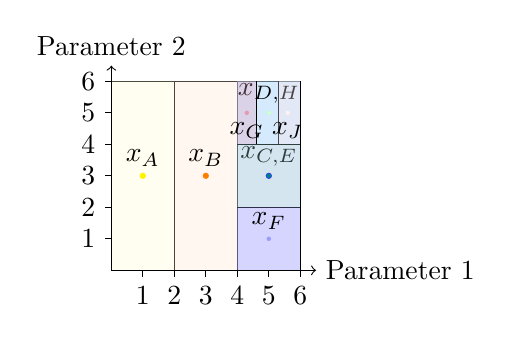
\begin{tikzpicture}[scale=0.4]

    % Define the grid
    \draw[step=6,black,very thin] (0,0) grid (6,6);

    
    % first decomposition
    \draw (2,0) -- (2,6) ;
    \draw (4,0) -- (4,6);
        % point A
        \fill[yellow!20, opacity = 0.3] (0.0,0) rectangle (2,6);
        \fill[fill = yellow] (1,3) circle (0.1) node[above]{$x_A$};  % Point in the first square
        
        % point B
        \fill[orange!20, opacity = 0.3] (2,0) rectangle (4,6);
        \fill[fill = orange] (3,3) circle (0.1) node[above]{$x_B$};  % Point in the first square
        % point C
        \fill[blue!20, opacity = 0.3] (4,0) rectangle (6,6);
        \fill[fill = blue] (5,3) circle (0.1) node[above]{$x_{C,E}$};  % Point in the first square

    % second decomposition
    \draw (4,2) -- (6,2);
    \draw (4,4) -- (6,4);
      % point D
      \fill[cyan!40, opacity = 0.3] (4,4) rectangle (6,6);
      \fill[fill = cyan!40] (5,5) circle (0.07) node[above]{$x_{D,H}$} ;  % Point in the first square
      %point E
      \fill[teal!40, opacity = 0.3] (4,2) rectangle (6,4);
      \fill[fill = teal] (5,3) circle (0.07) ;  % Point in the first square
      %point F
      \fill[blue!40, opacity = 0.3] (4,0) rectangle (6,2);
      \fill[fill = blue!40] (5,1) circle (0.07) node[above]{$x_F$} ;  % Point in the first square

    % second decomposition
    \draw (4.6,4) -- (4.6,6);
    \draw (5.3,4) -- (5.3,6);
      %point G
      \fill[purple!40, opacity = 0.3] (4,4) rectangle (4.6,6);
      \fill[fill = purple!40] (4.3,5) circle (0.07) node[below]{$x_G$} ;  % Point in the first square
      %point H
      %\fill[green!40, opacity = 0.3] (4.6,4) rectangle (5.3,6);
      \fill[fill = green!20] (5,5) circle (0.07);  % Point in the first square
      %point J
      \fill[pink!40, opacity = 0.3] (5.3,4) rectangle (6,6);
      \fill[fill = pink!20] (5.6,5) circle (0.07) node[below]{$x_J$} ;  % Point in the first square
    

    % Draw red points
    \fill[red] (3,3) circle (0.01);  % Point in the first square

    
    % Draw the axes
    \draw[->] (0,0) -- (6.5,0) node[right] {Parameter 1};
    \draw[->] (0,0) -- (0,6.5) node[above] {Parameter 2};
    
    % Add ticks and labels
    \foreach \x in {1,2,3,4,5,6} {
      \draw (\x,0) -- (\x,-0.2) node[below] {\x};
      \draw (0,\x) -- (-0.2,\x) node[left] {\x};
    }
    
\end{tikzpicture}